\subsection{Corriente de Bias y Tensión de Offset}

En un amplificador operacional ideal la impedancia de entrada es infinita, por lo que no habría corriente por la que pase por ella. Sin embargo, se debe reconocer que en un modelo real de un amplificador operacional su impedancia de entrada no es infinita, lo que significa la existencia de corrientes de entrada y tensión de offset. 

\begin{figure}[h]
    \centering
    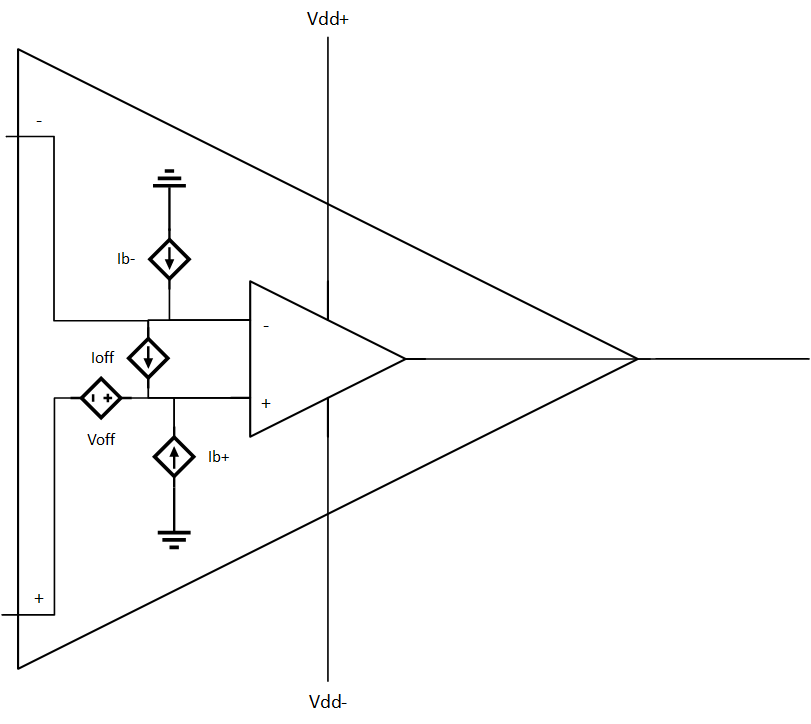
\includegraphics[scale = 0.4]{../Ejercicio2-MediciondeBias/Informe/modeloopamp.png}
    \caption{Modelo Real del Amplificador Operacional}
    \label{ej2opamp}
\end{figure}

\begin{itemize}
    \item Tensión de offset ($Voff$): 
    
    Sin la existencia de esta tensión parásita es lineal la determinación de la función de transferencia en un op-amp ideal con configuración inversa es:
    
    \begin{minipage}{.45\textwidth}
        \centering
        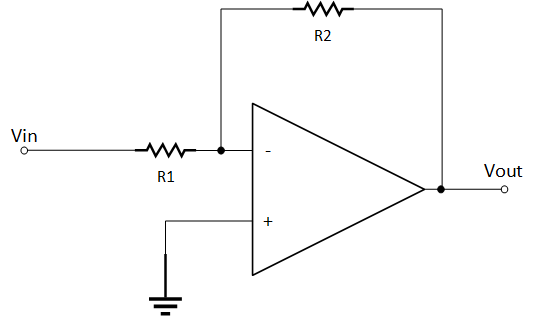
\includegraphics[scale = 0.5]{../Ejercicio2-MediciondeBias/Informe/inversopamp.png}
    \end{minipage}
    \begin{minipage}{.45\textwidth}
        $$H(s) = \frac{Vout}{Vin} = -\frac{R2}{R1}$$
    \end{minipage}

    Pero al tener la tensión de offset ($Voff$) de modo tal representado en la figura \ref{ej2opamp} obtenemos que:
    $$Vout = -Vin\frac{R2}{R1} + Voff\left(1 + \frac{R2}{R1}\right)$$
    Del cual observamos que dependiendo del valor de $Vin$ y $Voff$, el efecto de $Voff$ puede no ser despreciable, por ejemplo cuando:
    $$Vin = 0 \longrightarrow Vout = Voff \left(1 + \frac{R2}{R1}\right)$$
    
    \item Corrientes de Bias ($Ib$) y de offset ($Ioff$):
    
    Si bien estas corrientes no es querida dentro del circuito es esencial e inevitable esta porque es la que se encarga de polarizar el operador, en otras palabras que funcione de manera correcta el amplificador. Pero, a su vez introduce error en el sistema agregando una diferencia de tensión indeseada cuando halla una resistencia en seria en la entrada.
    
\end{itemize}

En consecuencia, es importante el análisis de las mismas para un realizar un diseño apropiado para la aplicación deseada conteniendo los errores mencionados. 

\vspace{3cm}

\subsection{Análisis del Circuito}

Se realiza las mediciones de las $Ib$, $Ioff$ y de $Voff$ sobre el siguiente circuito:

\begin{figure}[h]
    \centering
    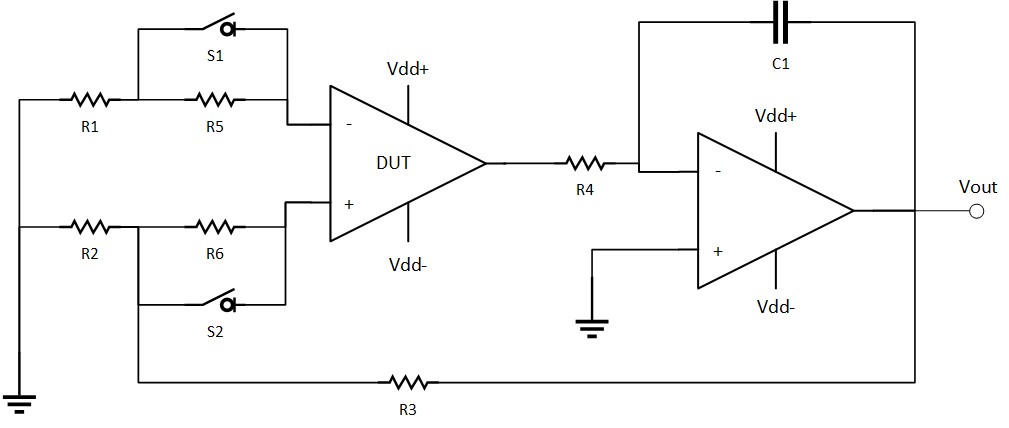
\includegraphics[scale = 0.65]{../Ejercicio2-MediciondeBias/Informe/circuito.png}
    \caption{Circuito de Medición de Corrientes y Tensiones de Offset}
    \label{ej2cir}
\end{figure}

Se aclara que el DUT es el op-amp a analizar, que en este caso es el TL081 y LF365; las resistencias utilizadas $R1 = R2 = 10\Omega \hspace{0.2cm} R3 = 3k\Omega \hspace{0.2cm} R4 = R5 = R6 = 100k\Omega$; y el capacitor $C1 = 1\mu F$

\subsubsection{Circuito de Realimentación}

Para conocer la operatividad del circuito se debe introducir el concepto de realimentación, circuito aquel en el que una muestra de la salida se superpone a la entrada con el propósito de controlar el comportamiento del sistema. 

\begin{figure}[h]
    \centering
    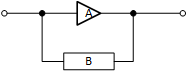
\includegraphics[scale = 1.5]{../Ejercicio2-MediciondeBias/Informe/realimentacion.png}
    \caption{Modelo de Realimentación}
    \label{ej2reali}
\end{figure}

Hay 2 categorías de circuitos de realimentación, produciendo los siguientes efectos:

\begin{itemize}
    \begin{minipage}{.49\textwidth}
         \item Negativa (fase de $\pi$ a $2\pi$ en relación a la entrada): 
        \begin{itemize}
            \item Disminuye de la ganancia efectiva del amplificador.
            \item Disminuye la impedancia de salida.
            \item Aumenta la impedancia de entrada.
            \item Aumento el ancho de banda.
            \item Disminuye el ruido.
            \item Reduce la distorsión no lineal.
            \item Mejora la estabilidad.
        \end{itemize}
    \end{minipage}
    \begin{minipage}{.45\textwidth}
        \item Positiva (fase de $0$ a $\pi$ en relación a la entrada): 
        \begin{itemize}
            \item Aumento de la ganancia efectiva del amplificador.
            \item Disminuye la impedancia de entrada.
            \item Disminuye el ancho de banda.
            \item Aumento la relación $\frac{se \tilde{n} al}{ruido}$, o sea ruido mayor.
            \item Puede conducir inestabilidad y auto-oscilaciones.
        \end{itemize}
    \end{minipage}
\end{itemize}

En este caso se utilizara una realimentación positiva cuya ecuación nos resulta:
$$x_i = x_A + x_B, \hspace{0.2cm} x_B = \beta x_A$$
$$y_o = A_{OL} x_i = A_{OL} (x_A + x_B) \Longrightarrow y_o - A_{OL} \beta y_o = A_{OL} x_i$$
$$H(s) = \frac{y_o}{x_i} = \frac{A_{OL}}{1-A_{OL}\beta}$$
Como en todos los amplificadores operacionales, se considera que la ganancia en lazo abierto $A_{OL}>>1$ o infinita, entonces la ganancia a lazo cerrado es:
$$A_{CL} = -\frac{1}{\beta}$$

\subsubsection{Funcionamiento del Circuito}

Teniendo 2 estapas dentro del circuito, comenzamos primeramente por la etapa de salida ya que de tal manera comprendemos la función del op-amp no analizado. Siendo $A_{vol}$ igual a la ganancia en lazo abierto del op-amp y considerando el capacitor en la realimentación, se obtiene la ganancia en lazo cerrado de esta etapa.

\begin{minipage}{.55\textwidth}
    \begin{center}
        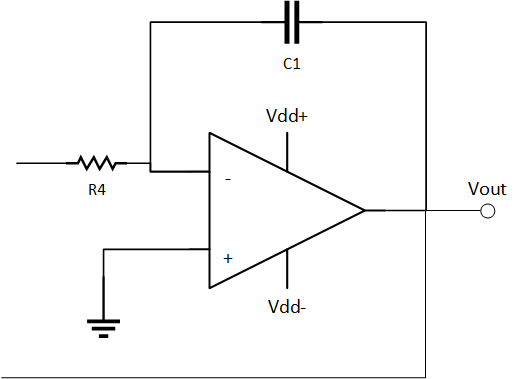
\includegraphics[scale = 0.5]{../Ejercicio2-MediciondeBias/Informe/etapa2.png}
        \captionof{figure}{Etapa de Salida: Amplificación Inversa}
        \label{ej2et1}    
    \end{center}
\end{minipage}
\begin{minipage}{0.45\textwidth}
    Ganancia a lazo cerrado sera:
    
    $$A_{CL} = \frac{-A_{vol}}{1 + sRCA_{vol}}$$
    
\end{minipage}

En esta etapa se amplifica la señal continua, de esta manera se aumenta la precisión en la medición de las corrientes y tensiones de offset, esto es requerido porque las señales que se quieren medir tienen una amplitud comparable con el ruido que pueda llegar a inducirse en el circuito. Esta precisión se logra ya que el estudio del circuito es en continua, con $f = 0Hz$, por lo que el capacitor $C1$ va a actuar como un circuito abierto, bloqueando cualquier realimentación proveniente de la salida de $Vout$ cuya frecuencia sea mayor a $f> 0Hz$.

Luego, en la etapa de entrada:

\begin{minipage}{.55\textwidth}
    \begin{center}
        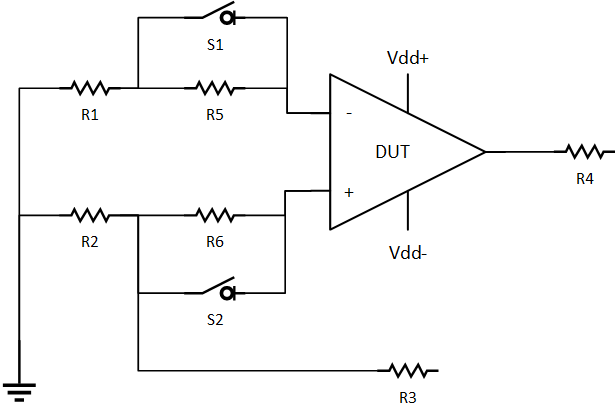
\includegraphics[scale = 0.5]{../Ejercicio2-MediciondeBias/Informe/etapa1.png}
        \captionof{figure}{Etapa de Entrada: Amplificación No Inversa}
        \label{ej2et2}
    \end{center}
\end{minipage}
\begin{minipage}{0.35\textwidth}
    
    La ganancia de una amplificación no inverso, considerando la retroalimentación $R3$ es:
    
    $$A_{CL} = \left( 1 + \frac{R3}{R2}\right) \Longrightarrow Vout_{DUT} = \left( 1 + \frac{R3}{R2}\right) Vin$$
    
    o a lazo abierto:
    
    $$A_{OL} = A_{vol}$$
\end{minipage}

Como mencionamos anteriormente, los amplificadores operacionales no son ideales, por lo que existen corrientes y tensiones parásitas que por consecuencia sucede que exista una tensión representada como:
$$Vin = (V^+ - V^-) = Voff + Ib^+ R5 - Ib^- R6$$
$$Ib = \frac{Ib^+ +  Ib^-}{2} \hspace{0.5 cm} Ioff = Ib^+ -  Ib^-$$
Se aclara que como en como $R1$ es relativamente chica, la diferencia de tensión que produce es casi nula por lo que $\Delta V_{R1} = Ib^- 10\Omega \approx 0$, análogamente $R2$. Sin embargo, cuando se abren los switch S1 o S2 existe una caída de tensión considerable por la resistencia $R5$ o $R6$.

Si queremos llevar los resultados obtenidos a la forma general de la retroalimentación positiva $H(s) = \frac{A_{OL}}{1-A_{OL}\beta}$ debemos analizar primeramente la ganancia total del lazo abierto del sistema. Para ello, concediéramos que la realimentación al sistema $\beta$ esta dada por la resistencia $R3$, de ello obtenemos la ganancia de lazo abierto como la multiplicación del lazo abierto de la etapa de entrada y el lazo cerrado de la etapa de salida, que para el sistema que concediéramos este lazo es coincidente al lazo abierto, por lo que nos queda:
$$A_{OL} = \frac{-A_{vol}^2}{1 + sRCA_{vol}}$$
Remplazando en la ecuación de realimentación la funcion de transferencia sera:
$$H(s)=\frac{-\frac{A_{vol}^2}{1+sRC\cdot A_{vol}}}{1+\frac{A_{vol}^2}{1+sRC\cdot A_{vol}}\beta}
	=-\frac{1}{\frac{1}{A_{vol}^2}+\beta}\cdot \frac{1}{\frac{s}{\frac{1+A_{vol}^2\beta}{RCA_{vol}}} +1}$$
Si se considera que $A_{vol}^2\beta >> 1$ se puede simplificar la expresi\'on:
	\[H(s) = -\frac{1}{\beta}\cdot \frac{1}{\frac{s}{\frac{A_{vol}\beta}{RC}}+1}\]
Considerando un modelo de polo dominante $\Longrightarrow A_{vol} = \frac{A_o}{\frac{s}{\omega_p}+1}$, donde $\omega_p = 2\pi \frac{BWP}{A_{vol}}$, tenemos:

    $$H(s) = -\frac{1}{\beta} \cdot \frac{1}{\frac{s}{\frac{\frac{A_o}{\frac{s}{\omega _p}+1}\beta}{RC}}+1}$$

$$H(s) = -\frac{1}{\beta} \cdot \frac{1}{s^2\frac{RC}{w_pA_o\beta}+s\frac{RC}{A_o\beta}+1}$$

Trayendo su forma a:
\begin{equation}
H(s) = \frac{1}{\frac{s^2}{\omega_0^2}+s\frac{2\xi}{\omega_0}+1}
\label{ej2FT}
\end{equation}
Resulta a un filtro pasa-bajos de segundo orden con:
$$\omega _0 = \sqrt{\frac{\omega_pA_o\beta}{RC}}$$
$$\xi=\frac{1}{2}\,\sqrt{\frac{\omega_pA_o\beta}{RC}}\,\frac{RC}{A_o\beta}=\frac{1}{2}\,\sqrt{\frac{\omega_pRC}{A_o\beta}}$$
Como la realimentación esta dada por $R3$ sabemos que $\beta = \frac{1}{\left(1 + \frac{R3}{R2}\right)} = \frac{1}{301} \Longrightarrow A_{CLideal} = -\frac{1}{\beta}$.

\subsection{Estudio de Resultados}

Se espera obtener resultados similares a la de la hoja de datos siendo:

\begin{table}[h]
\centering
\begin{tabular}{c|ccc|ccc}
\toprule
               & \multicolumn{3}{c|}{\textbf{TL081}}            & \multicolumn{3}{c}{\textbf{LF356}}    \\
               & \textbf{Voff[mV]} & \textbf{Ib[pA]} & \textbf{Ioff[pA])} & \textbf{Voff[mV]} & \textbf{Ib[pA]} & \textbf{Ioff[pA]} \\
\hline
Valor t\'ipico & 3            & 30        & 5         & 3            & 30    & 3     \\
Valor m\'aximo & 15            & 400       & 200       & 10           & 200   & 50   \\
\hline
\end{tabular}
\caption{Valores de las hojas de datos a $25^oC$}
\label{tab:ej2datasheet1}
\end{table}

\begin{itemize}
    \item  Medición de $Voff$:
    
    Para medir la tensión de offset es necesario eliminar las otras variables incógnitas, por lo que se cierran S1 y S2 provocando que la diferencia de tensión de entrada en ambos pines sea aproximadamente nula dando solo lugar a la tensión de offset parásita en juego. De esta manera se obtuvo que:
    $$Voff = -\frac{Vout}{\left( 1 + \frac{R3}{R2}\right)}$$
    Note que el negativo es de la función es porque luego de la ganancia en la etapa de salida se procede a la etapa de salida, donde amplifica inversamente, o analíticamente también es posible justificarlo con la función de trasferencia debido a que trabajamos a una frecuencia $f = 0Hz$ la ganancia es $H(s) = A_{CLideal} = -\frac{1}{\beta}$. 
        
    Los resultados obtenidos fuero:
    
    \begin{table}[h]
        \centering
        \begin{tabular}{cccc}
        \toprule
                \textbf{\begin{tabular}[c]{@{}c@{}}Entrada\\ (DUT)\end{tabular}} & \textbf{Salida}           & \textbf{\begin{tabular}[c]{@{}c@{}}Vout {[}mV{]}\end{tabular}} & \textbf{\begin{tabular}[c]{@{}c@{}}Voff {[}mV{]}\end{tabular}} \\
                \hline
                TL081                                                            & TL081                     & -43.754                                                          & 0.145                                                            \\
                
                TL081                                                            & LF356                     & -38.295                                                          & 0.127                                                            \\
                
                LF356                                                            & LF356                     & 429.7                                                            & -1.428                                                           \\
                
                LF356                                       & TL081 & 415.4                                       & -1.380 \\
                \hline
        \end{tabular}
    
    \end{table}
    
    \item Medición de $Ib$ y $Ioff$:
    
    Como luego de medir $Voff$ tenemos la tensión parásita que esta constantemente dentro del circuito es posible buscar las corrientes parásitas dentro del circuito.
    
    $Ib^+$ se podrá medir abriendo el switch S2 y cortocircuitado R5 y encontrar la relación:
    $$Ib^+ = \frac{1}{R6}\left(-\frac{Vout}{\left( 1 + \frac{R3}{R2}\right)}-Voff  \right) $$
    $Ib^-$ se podrá medir abriendo el switch S1 y cortocircuitado R6 y encontrar la relación:
    $$Ib^- = -\frac{1}{R5}\left( \frac{Vout}{\left( 1 + \frac{R3}{R2}\right)}+Voff  \right) $$    

    Luego al medir observamos:
    
% Please add the following required packages to your document preamble:
% \usepackage{booktabs}
% \usepackage{multirow}
\begin{table}[h]
\begin{tabular}{@{}ccccccccccc@{}}
\toprule
\textbf{\begin{tabular}[c]{@{}c@{}}Entrada\\ (DUT)\end{tabular}} & \textbf{Salida}            &                                                    & \textbf{Vout {[}mV{]}} & \textbf{Ib+{[}pA{]}}      & \textbf{}                                          & \textbf{Vout {[}mV{]}} & \textbf{Ib-{[}pA{]}}       & \textbf{}                              & \textbf{|Ib{[}pA{]}|} & \textbf{|Ioff{[}pA{]}|} \\ \midrule
TL081                                                            & \multicolumn{1}{c|}{TL081} & \multicolumn{1}{c|}{\multirow{4}{*}{\textbf{Ib+}}} & -31.996                & \multicolumn{1}{c|}{-387} & \multicolumn{1}{c|}{\multirow{4}{*}{\textbf{Ib-}}} & -34.154                & \multicolumn{1}{c|}{-315}  & \multicolumn{1}{c|}{\multirow{4}{*}{}} & 351                   & 72                      \\
TL081                                                            & \multicolumn{1}{c|}{LF356} & \multicolumn{1}{c|}{}                              & -32.77                 & \multicolumn{1}{c|}{-181} & \multicolumn{1}{c|}{}                              & -29.99                 & \multicolumn{1}{c|}{-274}  & \multicolumn{1}{c|}{}                  & 227.5                 & 93                      \\
LF356                                                            & \multicolumn{1}{c|}{LF356} & \multicolumn{1}{c|}{}                              & 419.7                  & \multicolumn{1}{c|}{336}  & \multicolumn{1}{c|}{}                              & 449.8                  & \multicolumn{1}{c|}{-663}  & \multicolumn{1}{c|}{}                  & 163.5                 & 999                     \\
LF356                                                            & \multicolumn{1}{c|}{TL081} & \multicolumn{1}{c|}{}                              & 410                    & \multicolumn{1}{c|}{179}  & \multicolumn{1}{c|}{}                              & 446.4                  & \multicolumn{1}{c|}{-1031} & \multicolumn{1}{c|}{}                  & 426                   & 1201                    \\ \bottomrule
\end{tabular}
\end{table}

\end{itemize}
    
Como podemos observar, si bien existe una diferencia al utilizar amplificador desiguales en la etapa de salida pero es posible identificar que los rázagos dominantes a la salida son las del DUT, o sea del amplificador a evaluar. 

Por otra parte, al finalizar las mediciones de los dispositivos es notable la disparidad con los valores esperados, aunque los $Voff$ están dentro de los rangos esperados, las corrientes presentan una mayor desigualdad. Estas diferencias son posibles de ser justificadas por la temperatura que esta operando el sistema. Uno de las componentes afectadas por la temperatura es la resistencia, que a mayor temperatura estas generan mas ruido térmico. Otro es el amplificador que puede no estar operando a $25^o C$, es decir existe un mayor rango de error cuando se midieron las corrientes y tensiones, es por ello que el fabricante también incluye los datos del valor máximo de corriente $Ib$ e $Ioff$ del integrado operando dentro de la temperatura de trabajo que son:
\begin{table}[h]
\centering
\begin{tabular}{c|ccc|ccc}
\toprule
               & \multicolumn{3}{c|}{\textbf{TL081}}            & \multicolumn{3}{c}{\textbf{LF356}}    \\
               & \textbf{Voff[mV]} & \textbf{Ib[nA]} & \textbf{Ioff[nA])} & \textbf{Voff[mV]} & \textbf{Ib[nA]} & \textbf{Ioff[nA]} \\
\hline
Valor m\'aximo & 20           & 10   & 2    & 13            & 8       & 2       \\
\hline
\end{tabular}
\caption{Valores de las hojas de datos a rango entero}
\label{tab:ej2datasheet1}
\end{table}

De acuerdo a esta tabla los valores obtenidos de $Ib$ y $Ioff$ podemos notar que efectivamente pudo haber influido en la medición la temperatura al que estaban trabajando. 

Otro problema pudo ser provocado por la placa utilizada, esta es el Electronics Explorer que tiene un limite en la tensión que puede dar al amplificador operacional de $V_{dd} = \pm9V$, la cual difiere con las especificaciones dadas por el fabricante que se testeó a $V_{dd} = \pm 15$. Además, el Electronics Explorer en esencia es una protoboard, es decir una placa de testeo útil pero no son muy capaces cuando queremos mediciones precisas porque son mucho mas afectadas por el ruido externo e interno de la placa, esto nos lleva a mas errores durante la medición del circuito. 

\subsection{Evaluación del Circuito}

\subsubsection{Capacitor en Uso}

Como el circuito introducido es vulnerable al ruido es inevitable el uso de un capacitor para realizar una medición del bias. Sin embargo la cuesto es cual capacitor seleccionar, para ello debemos recurrir a la función de transferencia mencionada en la ecuación \ref{ej2FT}. De aqui encontramos que:
$$f_0=\frac{1}{2\pi}\cdot \sqrt{\frac{\omega_pA_o\beta}{RC}}$$
Teniendo en cuenta la información dada en la hoja de datos podemos calcular su frecuencia de corte:
% Please add the following required packages to your document preamble:
% \usepackage{booktabs}
\begin{table}[h]
\centering
\begin{tabular}{@{}ccc@{}}
\toprule
\textbf{}     & \textbf{TL081} & \textbf{LF365} \\ \midrule
$A_{vol}$          & 200            & 200            \\
BWP {[}MHz{]} & 3              & 5              \\
$\omega_p$ {[}kHz{]}   & 94             & 157            \\ \midrule
$f_0$ {[}Hz{]}    & 126            & 163           \\
\hline
\end{tabular}
\end{table}

Es decir que los ruidos que son de aproximadamente $50Hz$ no se encuentran atenuadas para nuestro circuito. Entonces, si se desea atenuar el ruido debemos tener una frecuencia de corte $f_0<50Hz$ necesitaríamos un capacitar de: 
$$C>\frac{\omega_pA_o\beta}{4\pi^2R(50Hz)^2}$$
Lo cual para el $TL081$ el capacitor debe valer $C > 6.3\mu F$ y para el $LF356$ uno de $C>10.6\mu F$.
 
\subsubsection{Estabilidad del Circuito}

Si se desea estudiar la estabilidad del circuito, nuevamente es esencial la función de transferencia de la ecuación \ref{ej2FT}. Por lo que se estudia las singularidades del sistema, o sea los polos del mismo.
$$S_{1,2} = \frac{-\frac{2\xi}{\omega_0}\pm\sqrt{\frac{4\xi^2}{\omega_0^2}-\frac{4}{\omega_0^2}}}{\frac{2}{\omega_0^2}}=-\omega_0\xi \pm {\omega_0}\sqrt{\xi^2-1}$$
Siendo $\omega_0\xi > {\omega_0}\sqrt{\xi^2-1}$ en ambos circuitos con los diferentes opamps, el sistema resulta estable por tener los polos con parte real negativa. 

\subsubsection{Configuraciones}

\begin{itemize}
    \item Inversión las entradas:
    
    Si se invierten las entradas de los amplificadores, su amplificación en el sistema sufre leves alteraciones, cambiando el producto final de la función de transferencia. 
    
    \begin{itemize}
        \item Invertir las entradas de la etapa de salida: En este caso la amplificación a lazo cerrado del circuito cambiara a:
        \item Invirtiendo las entradas de ambas etapas: Cuando se realiza esta acción sucede que:
        $$A_{CL} = \frac{A_{vol}}{1 - sRCA_{vol}} \Longrightarrow A_{OL} = \frac{A_{vol}^2}{1 - sRCA_{vol}}$$
        Además, como ahora la entrada es una etapa de amplificación inversa:
        $$\beta = -\frac{1}{\frac{R3}{R1}} = -\frac{1}{300}$$
    \end{itemize}
    
    \item Circuito de compensación:
    
    Es posible la compensación de las tensiones de offset con ciertas configuraciones. Para este caso los propios fabricantes mencionan en la hoja de datos los siguientes circuitos con resistencias variables como muestran las siguientes figuras:
    
    \begin{minipage}{.4\textwidth}
    \begin{center}
        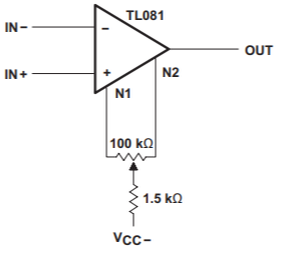
\includegraphics[width = 0.5\textwidth, height = 4cm]{../Ejercicio2-MediciondeBias/Informe/comptl081.png}
        \captionsetup{justification=centering}
        \captionof{figure}{Compensación de offset del TL081 con $R = 100k\Omega$}
        \label{ej2comp081} 
    \end{center}
    \end{minipage}
    \hspace{0.5cm}
    \begin{minipage}{.4\textwidth}
    \begin{center}
        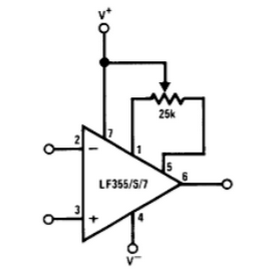
\includegraphics[width = 0.5\textwidth, height = 4cm]{../Ejercicio2-MediciondeBias/Informe/complm365.png}
        \captionsetup{justification=centering}
        \captionof{figure}{Compensación de offset del LF365 con $R = 25k\Omega$}
        \label{ej2comp365} 
    \end{center}
    \end{minipage}
    
    Otra compensación posible es en las corrientes de bias para los circuitos de amplificación inversa como:
    
    \begin{center}
        \begin{minipage}{0.7\textwidth}
            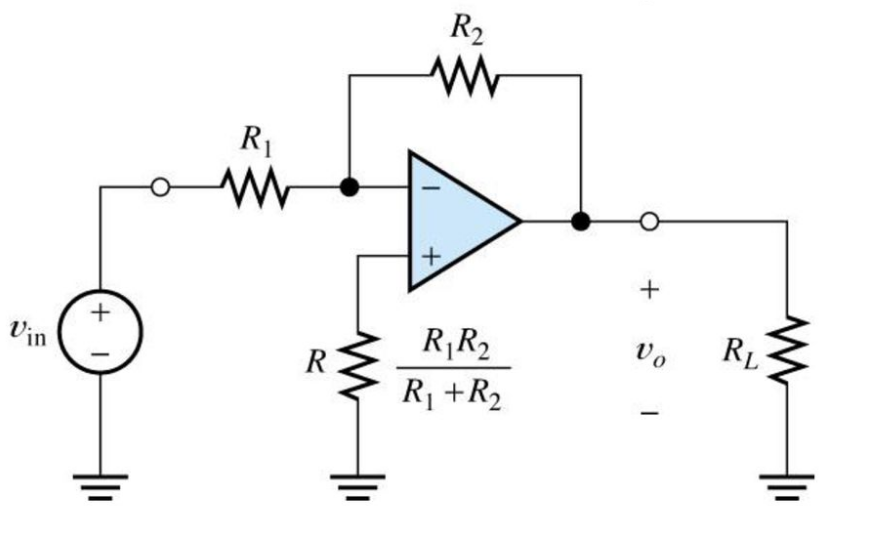
\includegraphics[scale = 0.4]{../Ejercicio2-MediciondeBias/Informe/compib.png}
        \captionsetup{justification=centering}
        \captionof{figure}{Compensación de Corriente de Bias}
        \label{ej2compib}
        \end{minipage}
    \end{center}
    
\end{itemize}